\documentclass[10pt]{beamer}
\usepackage{tikz}
\usepackage[utf8]{inputenc}


%Information to be included in the title page:
\title{Interleaved Quadrature and Optimization for Planning in Continuous State-Action Space}
\author{Nishad Gothoskar}
\institute{LIS}
\date{July 27 2018}
 
\begin{document}
 
\frame{\titlepage}
 
\begin{frame}
\frametitle{Value Function in RL: Discrete vs. Continuous}
Discrete
\begin{equation*}    % <--- deleted empty lines
        V^{\pi}(s) = \max_{a \in A} \Big[\sum_{s' \in S} p_{s'|s,a}(s'|s,a)\big(R(s'|s,a) + \gamma V^{\pi}(s')\big) \Big]
\end{equation*}
Continuous
\begin{equation*}    % <--- deleted empty lines
        V^{\pi}(s) = \max_{a \in A} \int_{s' \in S} p_{s'|s,a}(s'|s,a)\big(R(s'|s,a) + \gamma^{\Delta t}V^{\pi}(s')\big) \ \textup{d}s'
\end{equation*}
\newline
In our setting, this involves a maximization in a continuous action space, where the value of an action is an integral over the product of a continuous state space value function and the transition model. 
\end{frame}

\begin{frame}
\frametitle{Gaussian Process}
\begin{figure}
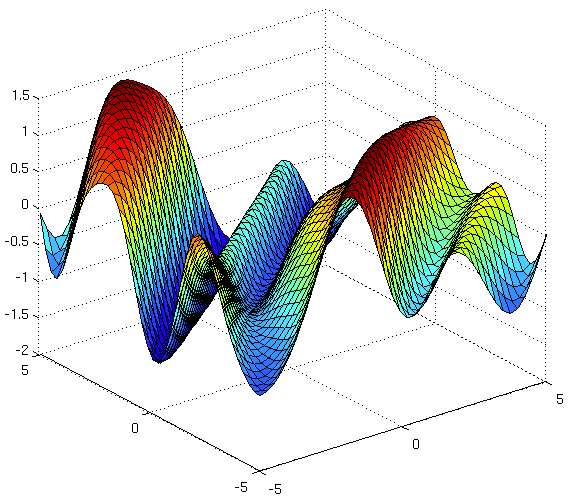
\includegraphics[scale=0.2]{gp}
\end{figure}
We will use a Gaussian Process to model the value function across our state space. With GPs, we define the value at certain support points and allow the model to generalize to other states. 
\newline  \newline
GPs also allow us to understand the distribution of value at a state, which we can use as a representation of our uncertainty about its value.
\begin{equation*}    % <--- deleted empty lines
	y^{*}|\bold{y} \sim \mathcal{N}(K_{*}K^{-1}\bold{y}, K_{**} - K_{*}K^{-1}K_{*}^{T})
\end{equation*}
\end{frame}

\begin{frame}
\frametitle{GP RTDP}
RTDP involves repeatedly iterating from start to goal state and then performing Bellman backup to update the value function.   
\newline  \newline
GPs also allow us to understand the distribution of value at a state, which we can use as a representation of our uncertainty about its value.
\begin{equation*}    % <--- deleted empty lines
	y^{*}|\bold{y} \sim \mathcal{N}(K_{*}K^{-1}\bold{y}, K_{**} - K_{*}K^{-1}K_{*}^{T})
\end{equation*}
\end{frame}
 
\end{document}

